\documentclass[tikz,border=0.1cm]{standalone}
\usepackage{tikz,tikz-3dplot}
\usepackage{amsmath,amsthm}
\usepackage{amssymb}
\usepackage{amsfonts}
\usepackage{xcolor}

\begin{document}
\newcommand{\Depth}{2}
\newcommand{\Height}{2}
\newcommand{\Width}{2}
\newcommand{\xxx}{0.39}
\newcommand{\yyy}{2.13}
\newcommand{\zzz}{1}

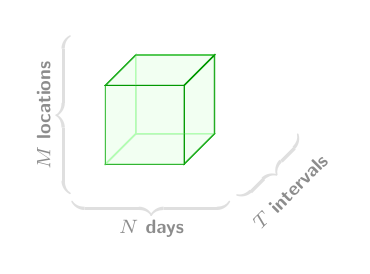
\begin{tikzpicture}[font=\sffamily]

\coordinate (O) at (0,0,0);
\coordinate (A) at (0,\Width,0);
\coordinate (B) at (0,\Width,\Height);
\coordinate (C) at (0,0,\Height);
\coordinate (D) at (\Depth,0,0);
\coordinate (E) at (\Depth,\Width,0);
\coordinate (F) at (\Depth,\Width,\Height);
\coordinate (G) at (\Depth,0,\Height);
\draw[green!60!black,fill=green!5] (O) -- (C) -- (G) -- (D) -- cycle;% Bottom Face
\draw[green!60!black,fill=green!5] (O) -- (A) -- (E) -- (D) -- cycle;% Back Face
\draw[green!60!black,fill=green!5] (O) -- (A) -- (B) -- (C) -- cycle;% Left Face
\draw[green!60!black,fill=green!5,opacity=0.8] (D) -- (E) -- (F) -- (G) -- cycle;% Right Face
\draw[green!60!black,fill=green!5,opacity=0.6] (C) -- (B) -- (F) -- (G) -- cycle;% Front Face
\draw[green!60!black,fill=green!5,opacity=0.8] (A) -- (B) -- (F) -- (E) -- cycle;% Top Face

\coordinate (O) at (0,0,0);
\coordinate (A) at (0,\Width,0);
\coordinate (B) at (0,\Width,\Height);
\coordinate (C) at (0,0,\Height);
\coordinate (D) at (\Depth,0,0);
\coordinate (E) at (\Depth,\Width,0);
\coordinate (F) at (\Depth,\Width,\Height);
\coordinate (G) at (\Depth,0,\Height);
\draw[green!30] (O) -- (C) -- (G) -- (D) -- cycle;% Bottom Face
\draw[green!30] (O) -- (A) -- (E) -- (D) -- cycle;% Back Face
\draw[green!30] (O) -- (A) -- (B) -- (C) -- cycle;% Left Face
\draw[green!60!black,opacity=0.8] (D) -- (E) -- (F) -- (G) -- cycle;% Right Face
\draw[green!60!black,opacity=0.6] (C) -- (B) -- (F) -- (G) -- cycle;% Front Face
\draw[green!60!black,opacity=0.8] (A) -- (B) -- (F) -- (E) -- cycle;% Top Face

\draw (0.2,-1.2,0) node {\scriptsize{\color{gray!90}\textbf{$N$~days}}};
\draw (0.2,-0.95,0) node[rotate = 0] {{\color{gray!25}$\underbrace{\hspace{2cm}}$}};
\draw (-0.4,1,2) node[rotate = 90] {\scriptsize{\color{gray!90}\textbf{$M$~locations}}};
\draw (-0.15,1,2) node[rotate = 270] {{\color{gray!25}$\underbrace{\hspace{2cm}}$}};
\draw (2.5,-0.2,1.4) node[rotate = 45] {\scriptsize{\color{gray!90}\textbf{$T$~intervals}}};
\draw (2.2,0,1.2) node[rotate = 45] {{\color{gray!25}$\underbrace{\hspace{1.1cm}}$}};

\end{tikzpicture}
\end{document}